\subsection{Rotation}
\paragraph{}An important consideration for this project is that the rotor is spinning at a high speed and this condition has to be somehow communicated to \textit{OpenFOAM}. To work with this condition there are three possible aproaches, which are widely described in \cite{Nozaki9240}, the Single Rotation Frame (SRF), the Multiple Reference Frame (MRF) and the Arbitrary Mesh Interference (AMI). In this particular case AMI is going to be used. The method itself is based on defining a sliding mesh where the part of the mesh that moves is rotating in every timestep and the values of the cells lying on the interference are interpolated to update the mesh in every timestep. 

\paragraph{}To apply this method, a solid containing the "moving" domain has to be defined as a \texttt{cellZone}. How to do that has been shown in the previous section. In our case the moving domain is the one contained between the low-pressure compressor and the nearest wall as shown in the figure~\ref{AMI}. 

\begin{figure}[h!]
\centering
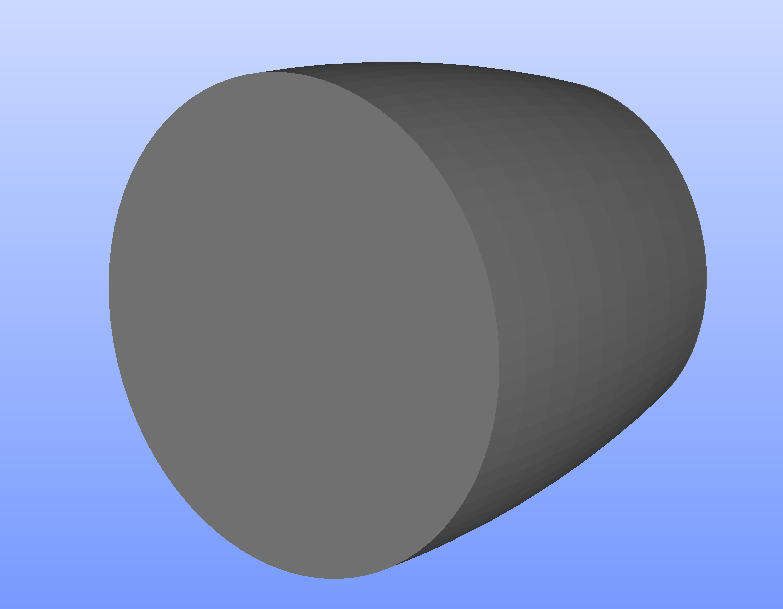
\includegraphics[scale=0.45]{./img/AMI.png}
\caption{Rotating zone solid}
\label{AMI}
\end{figure}

\paragraph{}To define the parameters related to the rotating zone such as the origin, the axis of rotation, the angular velocity and of course the zone which will be moving the \textit{constant/dynamicMeshDict} file has to be modified with the appropriate parameters for the case. Since the axis of \textit{OpenFOAM} are based on the right hand rule, the rotation axis must be defined as follows: \texttt{(1 0 0)}. From information found in different references, it has been chosen 5000 $rpm$ as the angular velocity of the rotor. It should be noted that the units used must be those of the International System, so the 5000 $rpm$ must be converted to $rad/s$. Furthermore, an origin point has to be indicated in the axis of rotation; in this case, the origin point is as follows: \texttt{(0 1.1675354 1.15542633)}. Finally the file will look like:


\begin{footnotesize}
\begin{verbatim}
/*--------------------------------*- C++ -*----------------------------------*\
| =========                 |                                                 |
| \\      /  F ield         | OpenFOAM: The Open Source CFD Toolbox           |
|  \\    /   O peration     | Version:  4.x                                   |
|   \\  /    A nd           | Web:      www.OpenFOAM.org                      |
|    \\/     M anipulation  |                                                 |
\*---------------------------------------------------------------------------*/
FoamFile
{
    version     2.0;
    format      ascii;
    class       dictionary;
    location    "constant";
    object      dynamicMeshDict;
}
// * * * * * * * * * * * * * * * * * * * * * * * * * * * * * * * * * * * * * //

dynamicFvMesh   solidBodyMotionFvMesh;

motionSolverLibs ( "libfvMotionSolvers.so" );

solidBodyMotionFvMeshCoeffs
{
    cellZone        innerAMI;

    solidBodyMotionFunction  rotatingMotion;
    rotatingMotionCoeffs
    {
        origin      (0 1.1675354 1.15542633);
        axis        (1 0 0);
        omega       523; // rad/s
    }
}


// ************************************************************************* //
\end{verbatim}
\end{footnotesize}

\paragraph{}Where \texttt{cellZone        innerAMI;} is used to define the rotating zone. It can clearly be seen that the modification of any parameter is pretty straigh-forward in the file since there is no possible confusion with the names. Another important thing to do when working with AMI is to define 2 patches related to this \textit{"moving zone"}. These patches can be created using the \textit{createPatch} routine. To do so, a dictionary (\textit{createPatchDict}) has to be included in the system folder. For this case, the dictionary file can be as follows:

\begin{footnotesize}
\begin{verbatim}
/*--------------------------------*- C++ -*----------------------------------*\
| =========                 |                                                 |
| \\      /  F ield         | OpenFOAM: The Open Source CFD Toolbox           |
|  \\    /   O peration     | Version:  2.3.1                                 |
|   \\  /    A nd           | Web:      www.OpenFOAM.org                      |
|    \\/     M anipulation  |                                                 |
\*---------------------------------------------------------------------------*/
FoamFile
{
    version     2.0;
    format      ascii;
    class       dictionary;
    object      createPatchDict;
}
// * * * * * * * * * * * * * * * * * * * * * * * * * * * * * * * * * * * * * //

// Do a synchronisation of coupled points after creation of any patches.
// Note: this does not work with points that are on multiple coupled patches
//       with transformations (i.e. cyclics).
pointSync false;

// Patches to create.
patches
(
    {
        //- Master side patch
        name            AMI1;
        patchInfo
        {
            type            cyclicAMI;
            matchTolerance  0.0001;
            neighbourPatch  AMI2;
            transform       noOrdering;
        }
        constructFrom patches;
        patches (AMI);
    }

    {
        //- Slave side patch
        name            AMI2;
        patchInfo
        {
            type            cyclicAMI;
            matchTolerance  0.0001;
            neighbourPatch  AMI1;
            transform       noOrdering;
        }
        constructFrom patches;
        patches (AMI_slave);
    }
);

// ************************************************************************* //
\end{verbatim}
\end{footnotesize}

\paragraph{}This method might seem more complicated than simply studying the case with MRF but the results obtained for this particular case are better with the scheme used in this report.